Hi-fidelity prototyperne valgte vi at lave på to forskellige måder. Den ene kaldet \emph{Prototype 1} ved hjælp af HTML, Javascript og CSS og den anden kaldet \emph{Prototype 2} som en Android applikation, der kører på en mobiltelefon. Med disse teknologier kunne vi styre præcist hvordan prototyperne skulle fungere, og det var forholdsvist hurtigt at lave forbedringer eller rettelser til hver især. Dog var det hurtigst at lave rettelser til prototype 1. Med disse teknologier kunne prototyperne testes på computer, tablet og mobiltelefon for at emulere hvordan vores scenarie for en håndboldkamp hang sammen. Grundidéen var at en person trackede en håndbold kamp, så derfor ville vedkommende højst sandsynligt sidde med et bærbart device ved sin side.\\\\Prototyperne gør det muligt at gennemgå en række tasks i et flow, der er bestemt på forhånd. For at beskrive flowet er det opstillet i rækkefølge nedenfor:
\begin{enumerate}
\item Indtast spillernavne for begge hold. (Task 1)
\item Drag and drop spillertrøje ind på de korrekte pladser. (Task 2)
\item Start kampen og godkend dermed at positionerne er korrekte. (Task 2)
\item Indtast de forskellige skudforsøg der opstår under kampen for hver spiller. (Task 3)
\item Afslut kampen når sidste fløjt går. (Task 3)
\item Se spillerstatistik og holdstatistik når kampen er slut. (Task 4)\\\\
\end{enumerate} 

\newpage
\subsection*{Visning af prototypen}
\addcontentsline{toc}{subsubsection}{Visning af prototypen}
For at imødekomme de forskellige designregler vi har haft om i kurset som f.eks. gestalt teori har vi arbejdet det ind i prototyperne. I gestalt er der regler om:
\begin{itemize}
\item Reglen om nærhed
\item Reglen om ensartethed
\item Reglen om lukkethed
\item Reglen om symbolik\\
\end{itemize}

\begin{figure}[ht!]
\centering
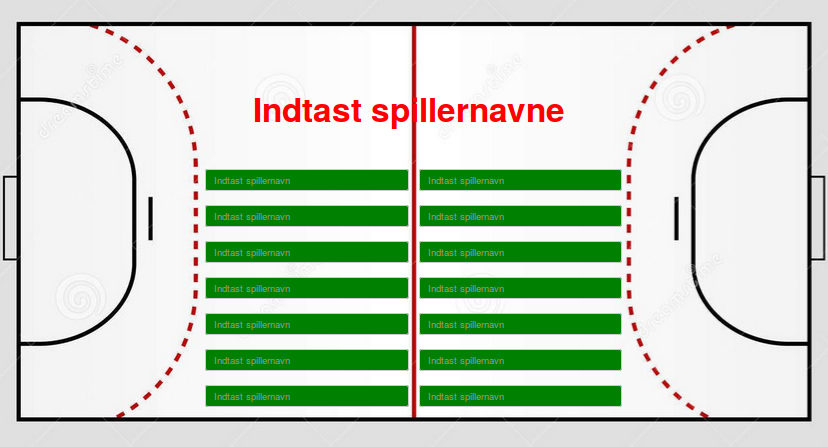
\includegraphics[width=150mm]{images/begin}
\caption{Prototype 1}
\end{figure}
På prototype 1 ses det hvordan vi har grupperet inputfelterne, så brugeren ved hvad der skal ske. De er for det første delt op i to grupper, så man let regner ud hvilke grupper der hører til hvilket hold. Alle felterne er ens, så man ved at det samme skal gøres med hvert felt. På grund af at vi har anvendt Bootstrap til vores CSS er inputfelterne lukket inde i en boks samtidig med at de med gestalt reglen om symbolik ligner noget brugeren har set før på internettet.\\\\

\newpage
På prototype 2 ses det ligeledes hvordan felterne er grupperet således de opfylder gestalt reglerne om nærhed, ensarthedhed samt symbolik, da de ligner andre input felter i Android applikationer. Som standard er felterne ikke lukkede af, men da skærmen er så lille ved brugeren at de hører sammen.
\begin{figure}[ht!]
\centering
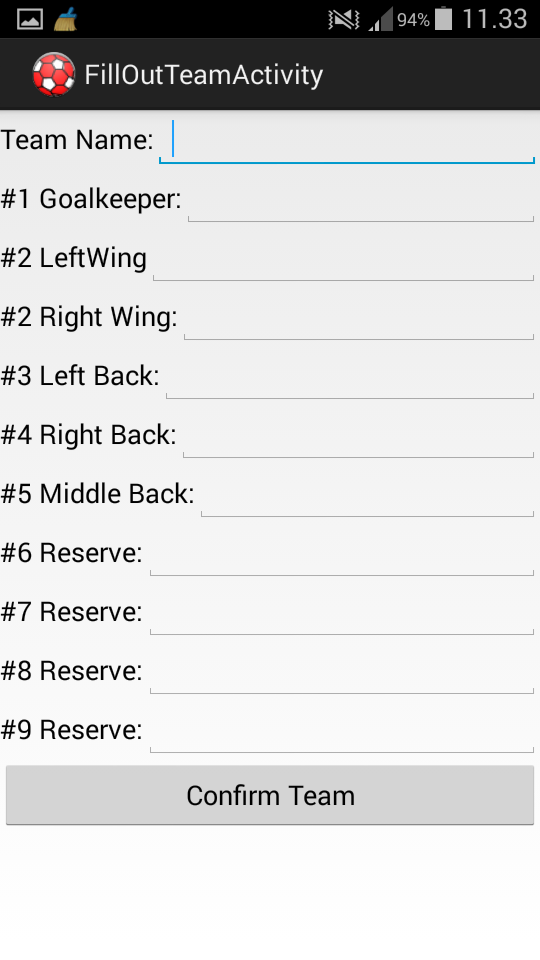
\includegraphics[width=50mm]{images/prototype2}
\caption{Prototype 2}
\end{figure}

\newpage
\subsection*{Peer review outcome}
\addcontentsline{toc}{subsubsection}{Peer review outcome}
Efter udvikling af prototyperne brugte vi andre personer til at teste dem for os. Dette blev gjort først for at se om brugere overhovedet kunne komme sikkert igennem prototyperne for at lave en binær statistik over dette. Det viste sig hurtigt at de brugere, der hjalp os, var ret kendte på disse typer af applikationer, hvilket nok skyldes de teknologier, der bruges og klassen var fuld af ingeniørstuderende.\\\\Eksempler på hvad vi fik ud af peer reviews:
\begin{itemize}
\item Det var farligt at komme til at dobbeltklikke på knapper, da man kom for langt i flowet.
\item Man kunne ikke gå baglæns i flowet.
\item Det er ikke sikkert der er præcis så mange personer på et hold.
\item Man kunne ikke se antal mål under kampen.
\item Screen scrolling er irriterende for brugeren.\\\\
\end{itemize} 

Den binære statistik viser hvordan brugerne klarede task 1 på prototyperne i forhold til hinanden.
\begin{figure}[ht!]
\centering
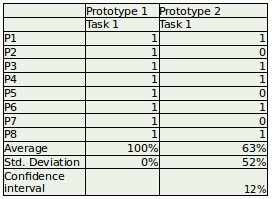
\includegraphics[width=100mm]{images/binary}
\caption{Binær data}
\end{figure}
Det ses at på prototype 1 kom alle igennem task 1, hvor på prototype 2 på mobiltelefonen, var det ikke all der kom igennem. Derfor opfyldte prototype 1 altså formålet langt bedre. Desuden kunne vi bruge de forskellige rettelser brugerne kom med til at forbedre prototypen, feks. ved at flytte knapper rundt, så man ikke dobbeltklikkede på dem.\\\\

\subsection*{Think aloud test}
\addcontentsline{toc}{subsubsection}{Think aloud test}
Da interaction design kan virke som en let forståelig opgave, er det vidt forskelligt hvordan mennesker opfatter brugergrænseflader i forhold til hinanden. Defor lavede vi en think-aloud test på prototype 1 for at se hvordan en uvedkommende person tænkte om prototypen. Her fandt vi blandt andet ud af at han genkendte designet fra andre lignende applikationer, men at han gerne ville se hvor mange mål han havde indtastet f.eks. i task 3.\\\\ 

\subsection*{Metrics and statistics}
\addcontentsline{toc}{subsubsection}{Metrics and statistics}
For at måle de to forskellige prototyper fra hinanden lavede vi statistik over time on task. 
\begin{figure}[ht!]
\centering
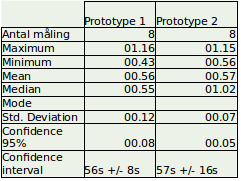
\includegraphics[width=100mm]{images/timeontask}
\caption{Time on task}
\end{figure}
Ved måling af dette var der umiddelbart ikke stor forskel på de forskellige prototyper, men som man kan se på statistikken er der forholdsvis stor afstand mellem max og min på prototype 1, hvilket gav en indikation af, at man måske kunne træne brugeren til at blive bedre i prototypen. Det gav anledning til at lave en learnability statistik over prototype 1.\\\\

\newpage
\begin{figure}[ht!]
\centering
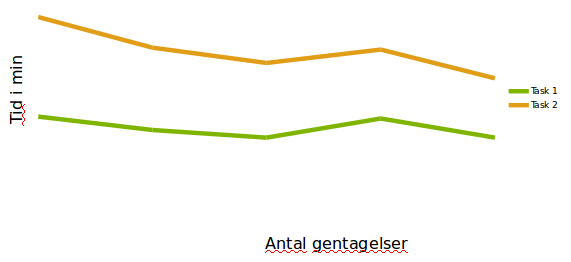
\includegraphics[width=100mm]{images/learnability}
\caption{Learnability curve}
\end{figure}
På kurven Learnability kurven ses det hvordan en bruger langsomt bliver hurtigere og hurtigere til at komme gennem prototypen. Og da det er en applikation, som brugeren gerne må bruge tid på inden en eventuel håndboldkamp er dette rigtig godt.



